\section{Mô hình hệ thống và phát biểu bài toán}
\label{sec:problem-formulation}

Khoảng trống nghiên cứu đặt ra câu hỏi rộng về khả năng duy trì chất lượng ISD khi mô
hình nền bị thu nhỏ. Để chuyển câu hỏi này thành một đối tượng mà harness có thể thao
tác, chúng tôi dùng constructive alignment để vận hành hoá sự nhất quán giữa các thành
phần của thiết kế giảng dạy.
Lựa chọn này không đồng nhất toàn bộ chất lượng ISD với alignment; nó cung cấp một thuộc
tính quan hệ trung tâm để hình thức hoá cơ chế và kiểm tra giả thuyết thiết kế.

\subsection{Mô hình hệ thống}
\label{sec:system-model}

\Cref{fig:architecture} mô tả ranh giới trách nhiệm giữa mô hình và harness. Mô hình
ngôn ngữ sinh nội dung; harness duy trì trạng thái, điều phối quy trình và thực hiện
kiểm soát chất lượng. Mọi thành phần của harness cùng đọc hoặc cập nhật một alignment
graph có phiên bản, đóng vai trò trạng thái thiết kế trung tâm.

\begin{figure*}[t]
  \centering
  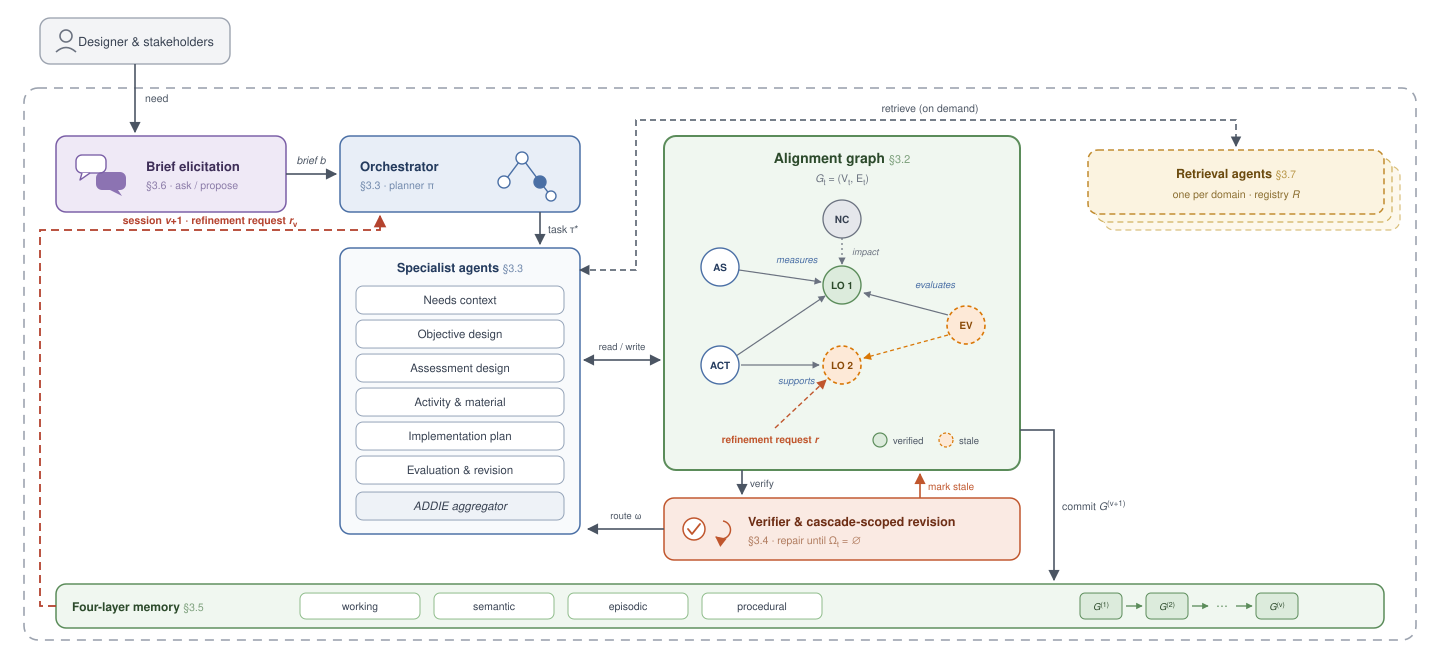
\includegraphics[width=\textwidth]{figures/architecture}
  \Description{Sơ đồ kiến trúc AlignmentGraph-ISD. Các tác tử chuyên biệt chạy theo
  thứ tự cố định và chỉ ghi những kiểu node, edge thuộc phạm vi của mình vào alignment
  graph. Sau mỗi lần ghi, tác tử kiểm chứng và sửa phần trạng thái do nó sở hữu. Bộ tổng
  hợp cuối cùng kết xuất chương trình ADDIE cùng artifact đồ thị phục vụ audit.}
  \caption{Kiến trúc AlignmentGraph-ISD. Các tác tử chuyên biệt lần lượt xây dựng
  alignment graph dưới phạm vi ghi giới hạn, rồi kiểm chứng và sửa lỗi ngay trong lượt
  của mình. Bộ tổng hợp cuối kết xuất chương trình ADDIE cùng artifact đồ thị auditable
  (\cref{sec:aggregation}). Mô hình nền có thể được thay thế mà không làm thay đổi các
  cơ chế của harness.}
  \label{fig:architecture}
\end{figure*}

\subsection{Alignment Graph}
\label{sec:alignment-graph}

Trong đầu ra dạng văn bản, quan hệ giữa các thành phần thiết kế chỉ tồn tại ngầm: người
đọc có thể nhận ra một assessment đang đo mục tiêu nào, nhưng hệ thống không có đối
tượng để kiểm tra quan hệ đó. AlignmentGraph-ISD giải quyết vấn đề này bằng cách hiện
thực hoá constructive alignment~\cite{biggs1996enhancing} thành cấu trúc dữ liệu tường
minh. Tại bước $t$, trạng thái thiết kế là đồ thị $G_t=(V_t,E_t)$. Tập đỉnh bao phủ các
thành phần thuộc năm pha ADDIE:
\begin{multline*}
V_t = V_{\mathrm{needs}} \cup V_{\mathrm{objective}} \cup V_{\mathrm{assessment}} \cup V_{\mathrm{activity}} \\
 \cup V_{\mathrm{material}} \cup V_{\mathrm{implementation}} \cup V_{\mathrm{evaluation}}.
\end{multline*}
Tập cạnh chỉ giữ ba quan hệ nhiều--nhiều trực tiếp phục vụ alignment:
\begin{align*}
E_t &= E_{\mathrm{measures}} \cup E_{\mathrm{supports}} \cup E_{\mathrm{evaluates}},\\
E_{\mathrm{measures}} &\subseteq V_{\mathrm{assessment}} \times V_{\mathrm{objective}},\\
E_{\mathrm{supports}} &\subseteq V_{\mathrm{activity}} \times V_{\mathrm{objective}},\\
E_{\mathrm{evaluates}} &\subseteq V_{\mathrm{evaluation}} \times V_{\mathrm{objective}}.
\end{align*}
Cạnh \textsl{measures} nối một assessment với mục tiêu mà nó đo; cạnh
\textsl{supports} nối một hoạt động với mục tiêu mà nó luyện tập; cạnh
\textsl{evaluates} nối một evaluation item với mục tiêu mà nó thẩm định. Quan hệ thứ ba
mở rộng bộ đôi activity--assessment quen thuộc để phù hợp với pha Evaluation của ADDIE:
việc đánh giá chương trình cũng phải quay lại các mục tiêu đã đặt ra. Các node
\texttt{needs}, \texttt{material} và \texttt{implementation} vẫn cần cho đầu ra ADDIE
hoàn chỉnh, nhưng không tham gia trực tiếp vào vị từ alignment; chúng được kiểm bằng các
ràng buộc khác, chẳng hạn tính khả thi của kế hoạch triển khai.

Mỗi mục tiêu học tập được biểu diễn bằng một node riêng
(\texttt{objective:LO-*}), nhờ đó hệ thống có thể kiểm tra alignment ở đúng đơn vị cần
được bảo đảm. Với mọi $o\in V_{\mathrm{objective}}$, điều kiện cấu trúc là:
\begin{multline}
\label{eq:aligned}
\mathrm{aligned}(o) \iff \big(\exists a\colon (a,o) \in E_{\mathrm{measures}}\big) \\
 \wedge \big(\exists x\colon (x,o) \in E_{\mathrm{supports}}\big) \wedge \big(\exists e\colon (e,o) \in E_{\mathrm{evaluates}}\big).
\end{multline}
\Cref{eq:aligned} mới xác nhận \emph{độ phủ cấu trúc}: mỗi mục tiêu có ít nhất một
liên kết thuộc từng loại. Constructive alignment còn đòi hỏi các liên kết đó hợp lệ về
nội dung và cấp độ nhận thức. Ví dụ, một assessment chỉ nhận biết khái niệm không thể
được xem là phép đo đầy đủ cho một mục tiêu yêu cầu phân tích. Verifier chịu trách nhiệm
kiểm tra lớp hợp lệ này (\cref{sec:qc}). Sau khi kiểm, cạnh được gắn cờ
\texttt{verified}; khi một node bị sửa, các node phụ thuộc có thể được đánh dấu
\texttt{stale} để buộc kiểm lại. Các trường này lưu dấu vết kiểm soát chất lượng trong
trạng thái chung.

Vị từ trong \cref{eq:aligned} đồng thời là tiêu chí thành công của bài toán, nên nó
cần được đo bằng một phép đo không phụ thuộc vào cơ chế nội bộ của harness. Thước đo
alignment trong \cref{sec:alignment-metric} lượng hoá trực tiếp cả hai lớp của vị từ
này---độ phủ cấu trúc và tính hợp lệ về nội dung, cấp độ nhận thức---trên đầu ra cuối
của \emph{mọi} hệ được so sánh, chỉ từ văn bản kết xuất. Nhờ đó, đại lượng được dùng để
định nghĩa thành công cũng chính là đại lượng được đo trong thực nghiệm (RQ2), thay vì
chỉ được xấp xỉ gián tiếp qua rubric chất lượng tổng quát.

\subsection{Ký hiệu và giả định}
\label{sec:assumptions}

\Cref{tab:notation} tóm tắt các ký hiệu. Chúng tôi giả định rằng: (i) design brief $b$
đã được cung cấp, còn quá trình hình thành brief nằm ngoài phạm vi; (ii) mô hình nền
không lưu trạng thái giữa các lượt và có thể được thay thế; (iii) đầu ra phải tuân theo
schema ADDIE của benchmark. Vì vậy, ADDIE là hợp đồng đầu ra, không phải yêu cầu duy nhất
đối với thứ tự thực thi bên trong harness.

\begin{table}[t]
  \caption{Ký hiệu.}
  \label{tab:notation}
  \small
  \begin{tabular}{@{}ll@{}}
    \toprule
    Ký hiệu & Ý nghĩa \\
    \midrule
    $b$ & design brief (input của harness) \\
    $G_t=(V_t,E_t)$ & alignment graph tại bước $t$ \\
    $o \in V_{\mathrm{objective}}$ & một learning objective (element node) \\
    $\mathrm{aligned}(o)$ & vị từ constructive-alignment, \cref{eq:aligned} \\
    $A_i$ & specialist agent cho concern ISD $i$ \\
    $V^{(i)},E^{(i)}$ & kiểu node/edge agent $i$ được ghi \\
    $\mathcal{V}$ & pedagogical verifier; $\Omega=\mathcal{V}(G)$ tập vi phạm \\
    $\rho,\gamma,\mu$ & hàm lấy context từ brief, graph, và bộ nhớ domain \\
    $M$ & bộ nhớ domain ổn định (ADDIE, Bloom, rubric template) \\
    $B$ & ngân sách lặp repair mỗi agent (\cref{sec:qc}) \\
    \bottomrule
  \end{tabular}
\end{table}

\subsection{Phát biểu bài toán}
\label{sec:problem-statement}

Với design brief $b$, mục tiêu là sinh một chương trình giảng dạy hoàn chỉnh, gồm đồ thị
$G$ và các thành phần ADDIE được kết xuất, sao cho:
\begin{enumerate}
  \item[(i)] mọi mục tiêu đều đạt độ phủ cấu trúc theo \cref{eq:aligned}, đồng thời
  các cạnh liên quan hợp lệ về nội dung và cấp độ nhận thức; và
  \item[(ii)] cơ chế duy trì chất lượng nằm trong harness và trạng thái alignment là
  tường minh, kiểm tra được bởi cả máy lẫn con người, với mục tiêu hạn chế mức suy giảm
  chất lượng khi mô hình nền được thu nhỏ. Mức độ đạt được mục tiêu này được kiểm tra
  bằng thực nghiệm trong \cref{sec:results}.
\end{enumerate}

\subsection{Thách thức}
\label{sec:challenges}

Bài toán khó vì ba lý do. Thứ nhất, alignment liên kết nhiều thành phần: không tác tử
nào chỉ nhìn phần đầu ra của mình có thể xác nhận toàn bộ điều kiện. Thứ hai, vi phạm
alignment thường không xuất hiện như một lỗi cục bộ; từng đoạn vẫn hợp lý dù các đoạn
không còn nhất quán với nhau. Thứ ba, nếu cơ chế kiểm soát chỉ nằm trong prompt, chất
lượng tiếp tục phụ thuộc vào khả năng tự tuân thủ của mô hình. Do đó, harness cần một
trạng thái chung có thể kiểm tra và một quy trình cập nhật tường minh.
